\section{Moto rettilineo uniformemente accelerato}
%---------------------------------------------------------------------------
In questo caso è l'accelerazione ad essere costante nel tempo
ne segue che:
\begin{equation}
    \vec a_{(t)} = \vec a_0 \quad\quad\quad \vec a_{(t)} = \frac{d\vec v}{dt} = 
    \frac{d^2\vec x}{dt^2}
\label{eq:acceleration}
\end{equation}
Per ricavare la legge oraria del moto uniformemente accelerato,
dobbiamo integrare due volte nel tempo, dato che l'accelerazione
è la derivata seconda del vettore $\vec x$.
\begin{multline}
    \vec v_{(t)} = \vec v_0 + \int_{t_0}^{t}dt' \vec a_{(t')} =  \vec v_0 +  \vec a_0\sx t - t_0\dx\seg
    \\\seg\boxed{\vec x_{(t)} = \vec x_0 +\vec v_0\sx t - t_0\dx + \frac12\vec a_0\sx t-t_0\dx^2}
\label{eq:MRUA}
\end{multline}

\subsection{Relazione tra velocità ed accelerazione in funzione dello spazio}
Ora vedremo un modo per legare le grandezze velocità ed 
accelerazione, considerando la loro dipendenza dalla posizione
invece che dal tempo.\\
In questo esempio però ci mettiamo nel sistema di riferimento 
in cui il moto si svolge lungo una retta, che chiameremo asse $x$.
\begin{equation}
    a = \frac{dv}{dt} = \frac{dv}{dx}\frac{dx}{dt} =
    v\frac{dv}{dx}\seg \int_{v_0}^{v}dv'v' = \int_{x_0}^{x}dx'a_{(x')}
\end{equation}
Se l'accelerazione non dipende dalla posizione $\sx a_{(x)} = a_0\dx$, otterremo:
\begin{equation}
    \boxed{v^2_{(x)} = v_0^2 + 2a_0\sx x-x_0\dx}
\label{eq:v(x)_0}
\end{equation}
Mentre in generale si avrà:
\begin{equation}
    \boxed{\boxed{v^2_{(x)} = v_0^2 + 2\int_{x_0}^x dx'a_{(x')}}}
\label{eq:v(x)_gen}
\end{equation}

\begin{figure}[htbp]
    \begin{center}
        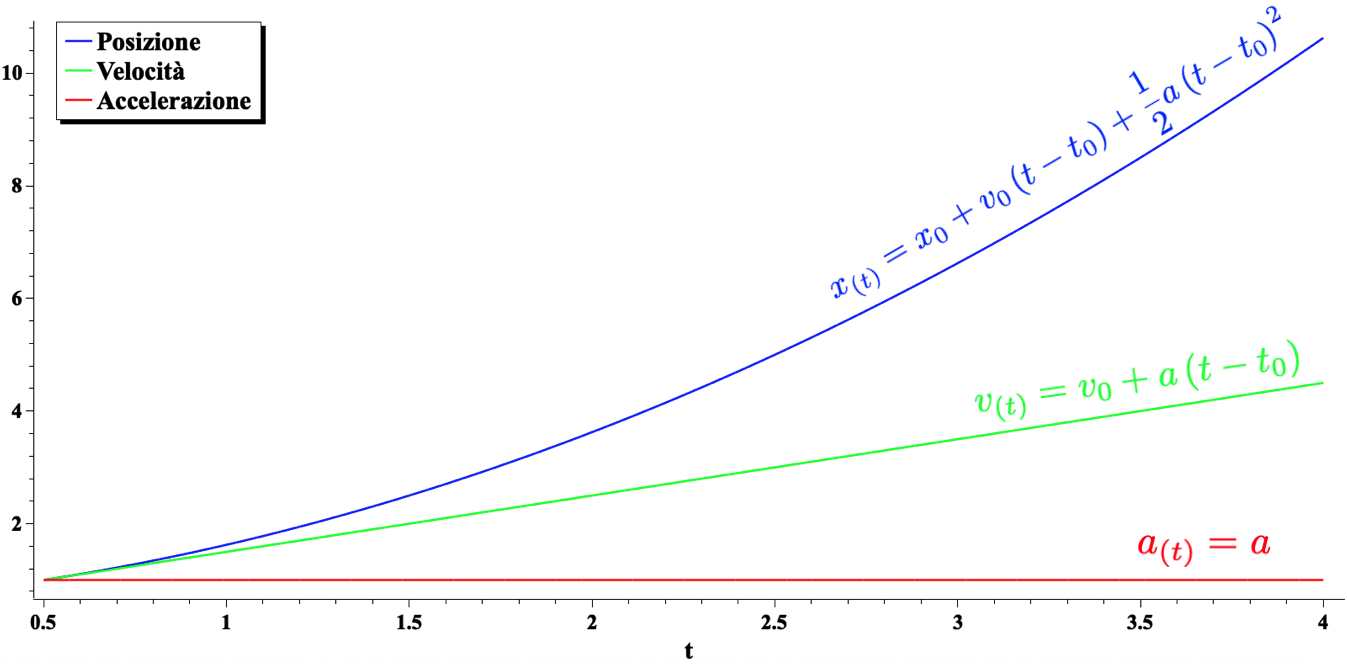
\includegraphics[width=13cm]{images/Motorettunifacc1.png} 
        \caption{Un esempio del grafico di accelerazione (rosso), velocità
        (verde) e posizione (blu), nel moto uniformemente accelerato
        unidimensionale. L'asse delle ascisse rappresenta il tempo,
        mentre quello delle ordinate la variabile dipendente.}       
    \end{center}
\label{fig:MRUA}
\end{figure}